\documentclass[letterpaper,12pt]{article}
\usepackage[utf8]{inputenc}

\usepackage{rotating}
\usepackage[top=1in, bottom=1in, left=1in, right=1in]{geometry}
\usepackage{graphicx}
\usepackage[numbers,square,sort&compress]{natbib}
\usepackage{setspace}
\usepackage[cdot,mediumqspace,]{SIunits}
\usepackage{hyperref}
\usepackage{mathtools}
\usepackage{url}
\usepackage{authblk}
\usepackage{placeins}
\usepackage{float}

\onehalfspacing
\title{Computational Physics Lab 10}
\author{Anita Bahmanyar}
\affil{\small {Student Number: 998909098}}
\date{November 14, 2014}

\usepackage{graphicx}

\renewcommand\thesubsection{\alph{subsection}}

\begin{document}

\maketitle

\section*{Q1}
The green box shows the boundary of the box so its easier to see that its not passing the boundary.

%figue a
\FloatBarrier
\begin{figure}[H]
\centering
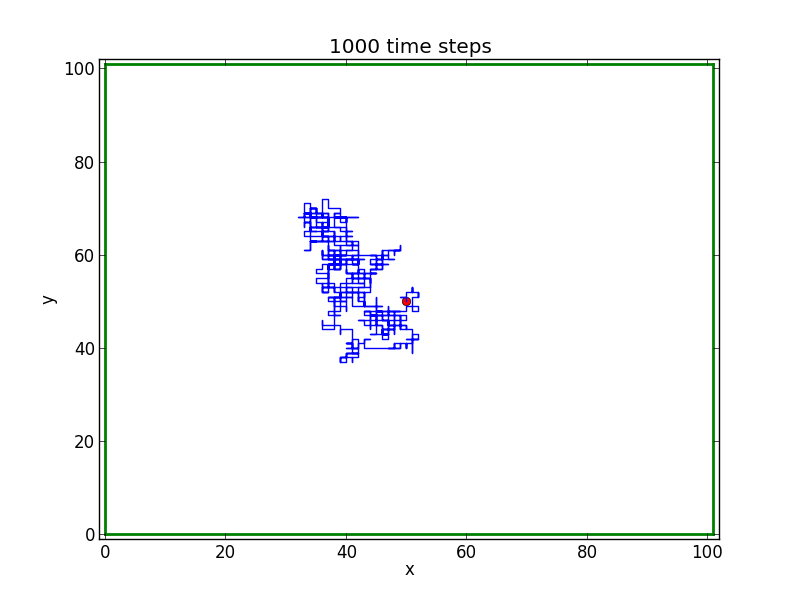
\includegraphics[scale=0.55]{q1a.png}
\caption{Random walk with 1000 time steps}
\end{figure}
\FloatBarrier

%figure b
\FloatBarrier
\begin{figure}[H]
\centering
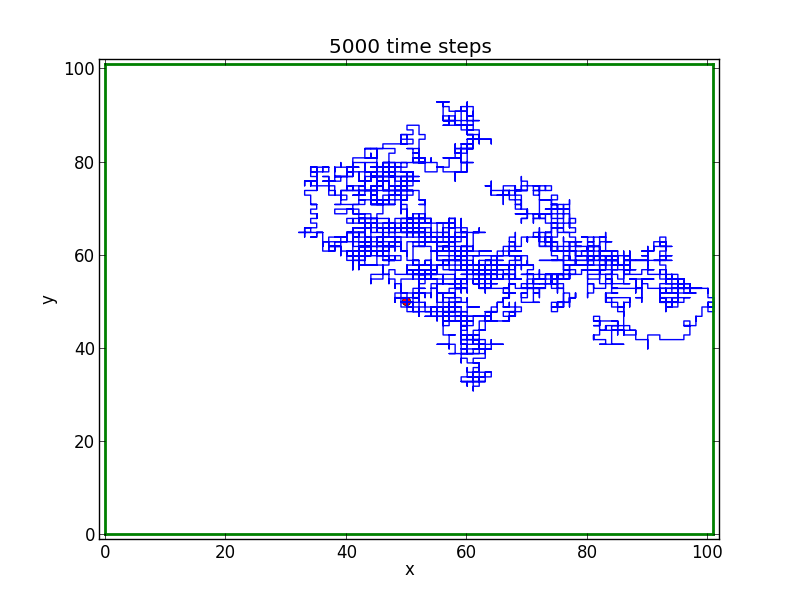
\includegraphics[scale=0.55]{q1b.png}
\caption{Random walk with 5000 time steps. This is hitting the boundary of the box but not crossing it which means the boundary conditions work.}
\end{figure}
\FloatBarrier


\section*{Q3}

\FloatBarrier
\begin{figure}[H]
\centering
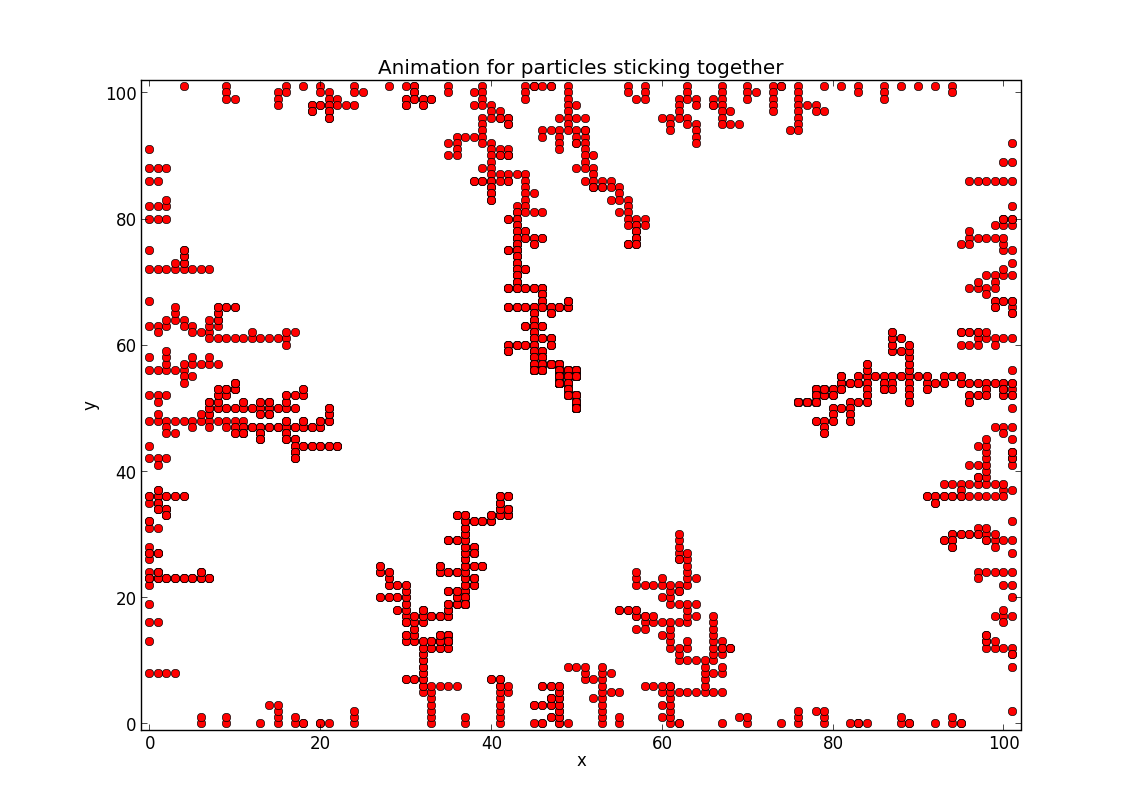
\includegraphics[scale=0.5]{q3.png}
\caption{This figure shows the position of particles attached to each other.}
\end{figure}
\FloatBarrier

\section*{Q4}
The integral value is 2.6112 $\pm$ 0.0001 . The way I calculated the error is by using equation in textbook:
\begin{equation}
\sigma = (b-a) \frac{\sqrt var f}{\sqrt N}
\end{equation}
where var f is defined as:
\begin{equation}
var f =\left \langle f^2 \right \rangle - \left \langle f \right \rangle ^2
\end{equation}
where

\begin{equation}
\left \langle f \right \rangle = \frac{1}{N} \sum_{i=1}^{N}(f(x_i))
\end{equation}

\begin{equation}
\left \langle f^2 \right \rangle = \frac{1}{N} \sum_{i=1}^{N} (f(x_i))^2
\end{equation}



\section*{Q6}

\FloatBarrier
\begin{figure}[H]
\centering
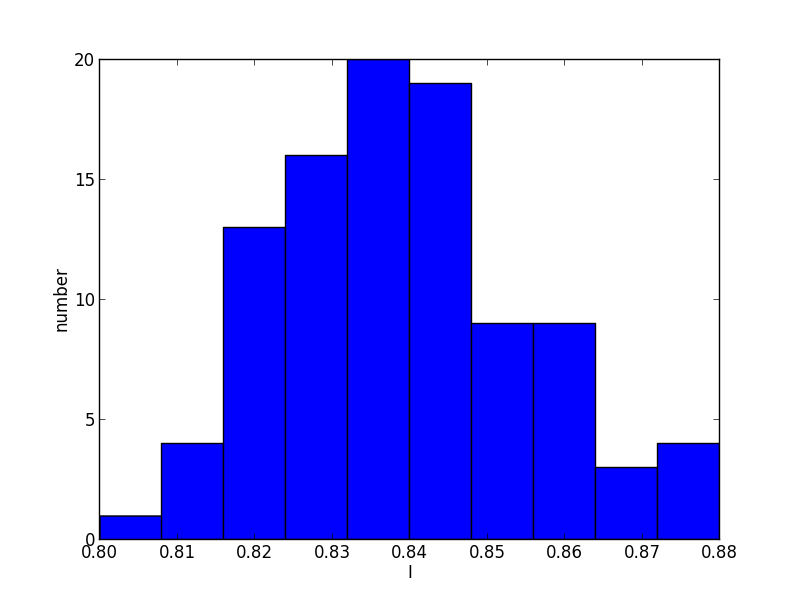
\includegraphics[scale=0.55]{q6.png}
\caption{Histogram of integral values using Mean value method.There is a peak which indicates the estimate for the value of integral but there is quite a lot of spread in the points.}
\end{figure}
\FloatBarrier

\section*{Q7}

\FloatBarrier
\begin{figure}[H]
\centering
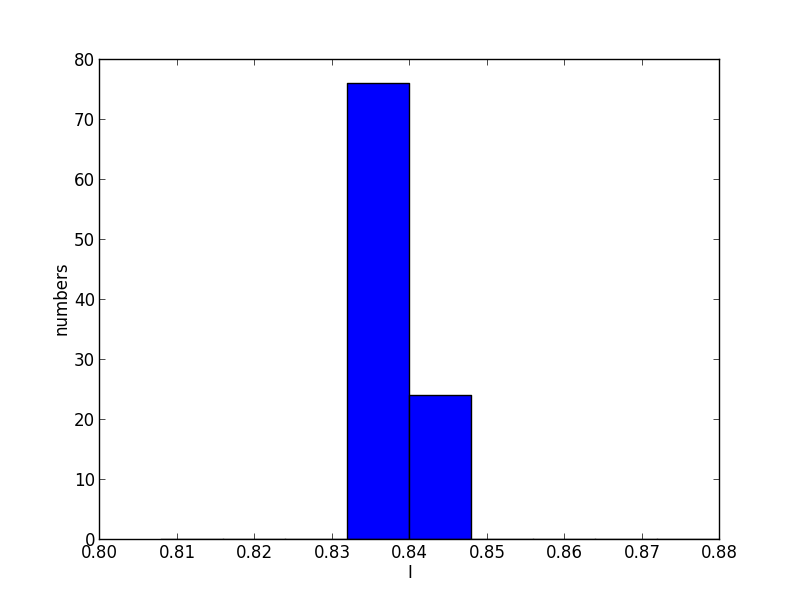
\includegraphics[scale=0.55]{q7.png}
\caption{Histogram of integral values using importance sampling method. This method uses non-uniform random numbers to estimate the integral values based on a given probability.}
\end{figure}
\FloatBarrier

As the histogram shows the method done in this question is much better than the method done in question 5 and 6, since the histogram has less spread in question 7, which means the value obtained is better.
\\In this question, I used the value of 2 for the $\int w$ by calculating it by hand. I also put the part in my code that calculates the integral of w using gaussian quadrature method and the value I got is 1.999 which is pretty close to the actual value, but using this value will introduce some error to the calculation of the integral. Therefore, importance sampling method is more precise than the mean value method.
\\ $\int \frac{1}{2 \sqrt x}= z $ so $\sqrt x = z$ and as a result, we have $x(z) =z^2$. Here, z values are uniformly random numbers between 0 and 1 and we can get  non-uniform random numbers by squaring the z values (which is based on the given probability in the question.)

\end{document}


